\thesischapter{How to use the class}

Use the provided directory structure for your content. Chapters and appendices should be
placed in directories called \texttt{chapterX} and \texttt{appendixX} respectively.\footnote{You
can use a different structure but this may break the word count and PDF builds on GitHub.}
Update \texttt{thesis.tex} where highlighted and build the PDF to create the thesis.

\thesissection{Package options}

\begin{description}[leftmargin=!,labelwidth=\widthof{\tt oneside}]
  \item[\texttt{oneside}] Double-sided is the default. Use the \texttt{oneside} option for
  a single-sided thesis.\footnote{Single-sided theses appear to be more common. A double-sided
  thesis includes blank pages to ensure that chapters start on the right (i.e. odd) page.
  These blank pages can however look odd when viewing as a PDF -- see the \texttt{pdf} option.}
  \item[\texttt{draft}] Use the \texttt{draft} option to add a word count, line numbers etc
  and enable to-do notes (see \cref{sec:todonotes}). Remove the draft option to create the
  final thesis for printing.
  \item[\texttt{pdf}] You may wish to also disseminate your thesis as a PDF. Use the \texttt{pdf}
  option to format the thesis for reading on screen.\footnote{Hyperlinks are shown in blue,
  pages with landscape tables/figures are rotated and blank pages inserted in two-sided
  theses are marked ``This page is intentionally blank''. Margins are equalised to remove the
  binding edge.}
  \end{description}

\thesissection{Thesis formatting}

\thesissubsection{Chapters and sections}\index{Formatting!chapters}\index{Formatting!sections}

Use the \verb|\thesischapter| command to create a new chapter. Sections and sub-sections
are created using \verb|\thesissection| and \verb|\thesissubsection| respectively.
Chapter and section titles will be converted to Title Case when using these commands.
Alternatively, the usual \verb|\chapter|, \verb|\section| and \verb|\subsection| commands
work as normal.

\thesissubsection{Tables and figures}\index{Formatting!tables}\index{Formatting!figures}

Include tables and figures in the usual way. Captions should be placed at the bottom.
\LaTeX\ will look in the \texttt{images/} and \texttt{figures/} directories for graphics.

\begin{figure}[h]
  \centering
  \begin{subfigure}[t]{0.3\textwidth}
    \includegraphics[width=\textwidth]{example-image-a}
    \caption{A sub-figure\dots}
    \label{fig:test-a}
  \end{subfigure}
  \begin{subfigure}[t]{0.3\textwidth}
    \includegraphics[width=\textwidth]{example-image-b}
    \caption{\dots another\dots}
    \label{fig:test-b}
  \end{subfigure}
  \begin{subfigure}[t]{0.3\textwidth}
    \includegraphics[width=\textwidth]{example-image-c}
    \caption{\dots and another}
    \label{fig:test-c}
  \end{subfigure}
  \caption{Example figure with three sub-figures. Larger margins and a smaller font are
  used to help distinguish captions from the main text.}
  \label{fig:test}
\end{figure}

\begin{table}[h]
  \centering
  \begin{tabular}{l r r r r}
  \toprule
  & Metric A & Metric B & Metric C & Metric D\\
  \midrule
  Model A & 10.431 & 0.154 & 0.715 & 28.871\\
  Model B & 25.488 & 0.279 & 0.190 & 14.992\\
  Model C & 14.992 & 0.396 & 0.280 & 20.947\\
  Model D & 20.947 & 0.362 & 0.412 & 20.558\\
  Model E & 21.137 & 0.006 & 0.411 & 2.665\\
  Model F & 19.445 & 0.513 & 0.242 & 16.087\\
  \bottomrule
  \end{tabular}
  \caption{Example table. Tables are formatted with \texttt{booktabs} and additional spacing
  between rows.}
  \label{tbl:test}
\end{table}

\thesissubsection{Mathematics}\index{Formatting!equations}\index{Formatting!theorems}

Use the \verb|\vect|, \verb|\matr| and \verb|\tens| commands to format vectors, matrices and
tensors respectively. These are all bold italic by default ($\vect{x}$, $\matr{X}$ and $\tens{X}$
respectively) and can be customised from lines 176 in \texttt{simple-thesis.cls}. The \href{https://ctan.org/pkg/isomath}{\texttt{isomath}}
package is used to comply with ISO 80000-2 e.g. sans-serif tensors.

The \href{https://ctan.org/pkg/amsmath}{\texttt{amsmath}}, \href{https://ctan.org/pkg/amssymb}{\texttt{amssymb}}
and \href{https://ctan.org/pkg/amsthm}{\texttt{amsthm}} packages are used to typeset equations
and theorems:

\begin{equation}
  f(x) = \frac{1}{\sigma\sqrt{2\pi}} \exp\left( -\frac{1}{2}\left(\frac{x-\mu}{\sigma}\right)^{\!2}\,\right)
\end{equation}

\newtheorem{theorem}{Theorem}
\begin{theorem}
  Your theorem here.
\end{theorem}
\begin{proof}
  Your elegant proof.
\end{proof}

\thesissubsection{Cross-references}\index{Formatting!cross-references}

Insert cross-references using \verb|\cref{label}| for ``\cref{fig:test}'' or \verb|\Cref{label}|
for a capitalised reference e.g. ``\Cref{fig:test}''. Sub-figures can also be referenced
e.g. \cref{fig:test-a}. See \href{https://ctan.org/pkg/cleveref}{\texttt{cleveref}} for more
information.

\thesissubsection{Bibliography}

The \texttt{biblatex}\footnote{See \url{https://www.overleaf.com/learn/latex/Bibliography_management_with_biblatex}.}
bibliography management package is used. Update \texttt{refs.bib} and use \verb|\cite{}|
or \verb|\parencite{}| to insert a numbered reference e.g. \cite{lecun_deep_2015}. Author
names can be included using \verb|\textcite{}| e.g. ``\textcite{lecun_deep_2015} state that \dots''.
The default citation style is \texttt{numeric-comp}\footnote{See \url{https://www.overleaf.com/learn/latex/Biblatex_citation_styles}.}
which is similar to IEEE but compressed e.g. multiple authors show as ``\textit{et al.}''
and multiple citations as [1, 2] or [1-3]. The bibliography style is \texttt{IEEE}\footnote{See \url{https://www.overleaf.com/learn/latex/Biblatex_bibliography_styles}.}.
These can be updated in \texttt{simple-thesis.cls}, see the ``Bibliography'' section.

\begin{sidewaysfigure}
  \centering
  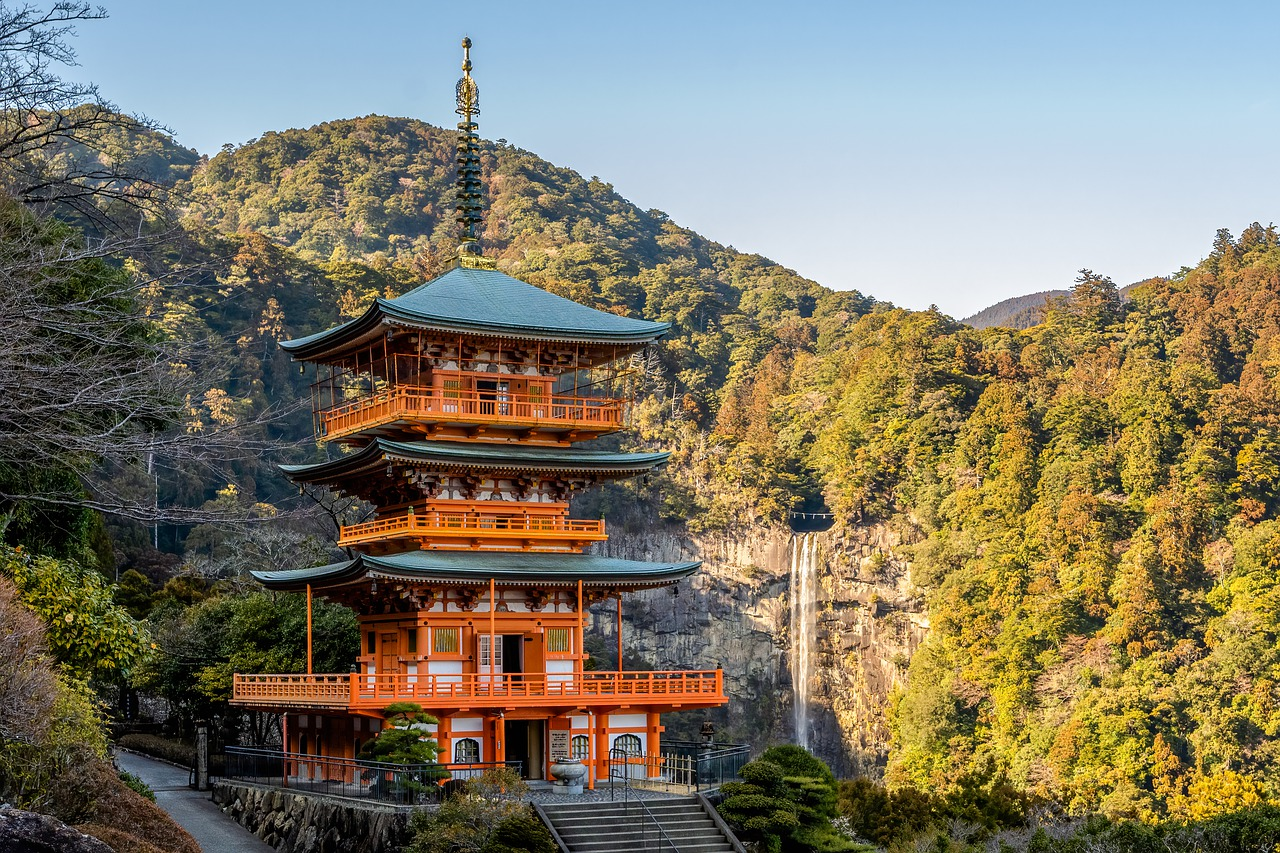
\includegraphics[width=0.7\textwidth]{pagoda}
  \caption{Example landscape figure (image by \href{https://pixabay.com/users/pen_ash-5526837/?utm_source=link-attribution&amp;utm_medium=referral&amp;utm_campaign=image&amp;utm_content=7868621}{Penny}
  from \href{https://pixabay.com//?utm_source=link-attribution&amp;utm_medium=referral&amp;utm_campaign=image&amp;utm_content=7868621}{Pixabay}).
  Newcastle University thesis guidelines state the ``\textit{top of tables/figures printed sideways
  should align to the left of the page}''. The \texttt{rotating} package aligns them centrally and
  a bug prevents changing this (easily). If this is important to you, a workaround is to add
  \texttt{\textbackslash vspace\{Xmm\}\textbackslash hspace\{0pt\}} below the caption. Adjust
  \texttt{X} to push the table/figure up to the correct position.}
  \label{fig:landscape}
  \vspace{7mm}\hspace{0pt}
\end{sidewaysfigure}

\begin{sidewaystable}
  \centering
  \begin{threeparttable}
    \begin{tabular}{l l r r r r r r r r r r}
    \toprule
    & & Metric A & Metric B & Metric C\tnote{1} & Metric D & Metric E & Metric F & Metric G\tnote{2} & Metric H & Metric I & Metric J\\
    \midrule
    \multicolumn{12}{l}{\textit{Results on first data set\tnote{3}}}\\
    & Model A & 0.226 & 0.101 & 10.233 & \textbf{26.374} & \textbf{24.131} & \textbf{0.088} & \textbf{10.431} & 0.154 & 0.715 & 28.871\\
    & Model B & 0.141 & 0.639 & 2.667 & 5.598 & 21.113 & 0.116 & 25.488 & 0.279 & \textbf{0.190} & \textbf{14.992}\\
    & Model C\tnote{4} & 0.416 & 0.992 & \textbf{29.190} & 12.098 & 16.279 & 0.127 & 14.992 & \textbf{0.396} & 0.280 & 20.947\\
    & Model D & \textbf{0.107} & \textbf{0.033} & 4.021 & 19.004 & 17.760 & 0.388 & 20.947 & 0.362 & 0.412 & 20.558\\
    \multicolumn{12}{l}{\textit{Results on second data set}}\\
    & Model A & 0.597 & 0.319 & 22.949 & 5.168 & \textbf{23.286} & 0.569 & 21.137 & 0.006 & 0.411 & \textbf{2.665}\\
    & Model B & \textbf{0.157} & 0.365 & 25.848 & 12.653 & 20.702 & \textbf{0.180} & 19.445 & 0.513 & \textbf{0.242} & 16.087\\
    & Model C\tnote{4} & 0.707 & \textbf{0.181} & 26.791 & 15.969 & 17.307 & 0.129 & 17.946 & 0.553 & 0.695 & 19.445\\
    & Model D & 0.496 & 0.861 & \textbf{26.956} & \textbf{20.050} & 13.525 & 0.272 & \textbf{2.665} & \textbf{0.902} & 0.291 & 7.472\\
    \bottomrule
    \end{tabular}
  \begin{tablenotes}
    \item[1] A note about metric C.
    \item[2] A note about metric G.
    \item[3] Caveat about the first data set.
    \item[4] Important point about model C.
  \end{tablenotes}
  \end{threeparttable}
  \caption{Example landscape table using \texttt{threeparttable} to add footnotes. Aligned
  using the same trick as \cref{fig:landscape} but centering the table would look better?}
  \label{tbl:landscape}
  \vspace{51mm}\hspace{0pt}
\end{sidewaystable}

\thesissubsection{Notation, acronyms and abbreviations}\index{Formatting!acronyms}\index{Formatting!notation}

\newacronym{nn}{NN}{neural network}

It is helpful to include a section with the definitions of any acronyms and abbreviations
used in your work. This is automated using \href{https://ctan.org/pkg/glossaries}{\texttt{glossaries}}.
When introducing a new acronym/abbreviation, define it with \verb|\newacronym{tag}{acronym}{definition}|\footnote{The 
definition should be lower case and singular.}, for example \verb|\newacronym{nn}{NN}{neural network}|.

The acronym is inserted using \verb|\gls{tag}|. The first instance of \verb|\gls{nn}| shows
as ``\gls{nn}''. Subsequent uses are abbreviated with a hyperlink to the glossary e.g. ``\gls{nn}''.
\verb|\Gls{tag}| capitalises the initial letter of the abbreviation, and \verb|\Glspl{tag}|
and \verb|\glspl{tag}| use the plural form.

The notation section is populated by adding definitions to \texttt{notation/notation.tex}.
The \texttt{name} is required for sorting but the \texttt{symbol} and \texttt{description}
are displayed, e.g.:
\begin{verbatim}
  \newglossaryentry{n}{
    name={N},
    description={Set of natural numbers \{0, 1, 2, \dots\}},
    symbol={\ensuremath{\mathbb{N}}}
  }
\end{verbatim}

\thesissubsection{Index}

An index is generated by including the \verb|\index{topic}| command when you discuss a topic.
Index entries can also have sub-items e.g. \verb|\index{topic!subtopic}|. The index includes
hyperlinks to the relevant page.

\thesissubsection{Quotes}\index{Formatting!quotes}

Enclose quotes between \verb|\begin{quote}[source]{author}| and \verb|\end{quote}|. The
\texttt{source} and \texttt{author} should be left empty if unused i.e. \verb|\begin{quote}[]{}|).

\begin{quote}[\href{https://www.tug.org/TUGboat/Articles/tb10-1/tb23knut.pdf}{Typesetting Concrete Mathematics}]{Donald E. Knuth}
  \dots there is a useful and meaningful distinction between text numerals and mathematical
  numerals. Text numerals are used in contexts like ``\oldstylenums{1776}'' and ``Chapter \oldstylenums{5}''\dots,
  where the numbers are essentially part of the English language; mathematical numerals, by contrast,
  are used in contexts like ``the greatest common divisor of 12 and 18 is 6'', where the numbers
  are part of the mathematics.
\end{quote}

\thesissubsection{Formatting numbers}\index{Formatting!numbers}

Note the difference between the two sets of numerals in the quote. Use \verb|\oldnum| for
``old style'' numerals (\oldnum{0123456789}). \verb|\num| formats ``lined'' numerals (0123456789)
for example with separating commas (\verb|\num{1234567.890123}| = \num{1234567.890123}) or 
scientific notation (\verb|\num{1.234e-5}| = \num{1.234e-5}). The
\href{https://ctan.org/pkg/siunitx}{\texttt{siunitx}} package can also typeset units.

\thesissubsection{University logo}\index{Formatting!title-page logo}

Replace \texttt{logo.png} in the \texttt{./images/} directory to update the title page logo.

\thesissection{To-do notes}\label{sec:todonotes}

To-do notes are provided by \href{https://ctan.org/pkg/todonotes}{\texttt{todonotes}}. Use:
\begin{itemize}
  \item \verb|\todonote{}| to create a to-do\todonote{This is a to-do note}
  \item \verb|\reference{}| to note a missing reference\reference{Need to add a reference here}
  \item \verb|\issue{}| to highlight a problem\issue{Need to fix this!}
  \item \verb|\misc{}| for a miscellaneous note\misc{This is a miscellaneous note}
\end{itemize}

When the \texttt{draft} package option is used, to-do notes are summarised on the first
page. All to-do notes are disabled when producing the final thesis. Text can also be 
\hl{highlighted} using \verb|\hl{}|. 

\thesissection{Building the PDF}\index{Building the PDF}

\thesissubsection{GitHub Actions}\index{Building the PDF!Using GitHub}

The thesis is built each time you push the repository to GitHub!\footnote{The main \texttt{.tex}
file must be named \texttt{thesis.tex}, and the \texttt{introduction/}, \texttt{chapterX/},
\texttt{conclusion/} directory structure must be followed.} Go to the \texttt{Actions}
tab, choose the commit (the top one is the most recent) and download by clicking \texttt{thesis-[TIMESTAMP]}
under \texttt{Artifacts}.

\thesissubsection{Locally}

Type \texttt{make} in the thesis directory to build the PDF.\footnote{This uses \texttt{latexmk}
to automate the build with the \texttt{pdflatex} engine, \texttt{biber} for references and
the glossary/index configuration in \texttt{.latexmkrc}.} This has been tested on
Ubuntu with TexLive\footnote{Ubuntu 18.04, 20.04 and 22.04 with TexLive installed using
\texttt{sudo apt install texlive-full}} and MacOS with MacTeX\footnote{MacOS Monterey 12.5.1
with MacTeX installed using \texttt{brew install --cask mactex-no-gui}}. If the document
fails to build, try \texttt{make purge} to delete all output and intermediate files\footnote{The
\texttt{make clean} command removes intermediate files only.}.

\texttt{make standalone} builds a standalone PDF for a single chapter. See the example
stub file \texttt{chapter1/chapter1-standalone.tex} which should be placed in each
chapter directory.

If you are unable to use \texttt{make} or \texttt{latexmk}, or prefer to use a recipe in
Visual Studio Code or TeXStudio:
\begin{enumerate}
  \item To generate the word count files run:\vspace{1ex}\\
    \texttt{\footnotesize texcount abstract/* *.tex -sum=1,0,1 -inc -out=wordcount.txt\\
    texcount abstract/* -sum=1,0,1 -1 -out=wordcount.abstract\\
    texcount introduction/* chapter*/* conclusion/* -sum=1,0,1 -brief -out=wordcount.summary\\
    texcount introduction/* chapter*/* conclusion/* -sum=1,0,1 -1 -out=wordcount.total}\\
  \item To generate the bibliography, acronyms and index sections run:\vspace{1ex}\\
    \texttt{\footnotesize pdflatex thesis.tex\\
    biber thesis\\
    makeglossaries thesis\\
    makeindex thesis}
  \item To build the final thesis, you will need to run \texttt{pdflatex thesis.tex} at least
    another two times to add all the sections and update the table of contents.
\end{enumerate}
